\chapter{प्रयोगशाला तकनीकें II: व्यवहार में संश्लेषण और विश्लेषण}\label{ch:b2:lab-techniques-2}

सोमवार की सुबह एक ग्रीन्यार अभिक्रिया विफल हो जाती है: फ़्लास्क को धोया गया था परंतु सुखाया नहीं गया था, और
उसमें बची जल की कुछ बूँदों ने अभिकर्मक को बनते ही नष्ट कर दिया। ओवन में सुखाए गए काँच के उपकरणों में,
नाइट्रोजन के अंतर्गत, विलोडित और ठंडे किए गए फ़्लास्क में हैलाइड को बूँद-बूँद मिलाकर फिर चलाने पर वही अभिक्रिया
सफल होती है। रसायन नहीं बदला; व्यवस्था बदली। यह अध्याय उस व्यवहार के बारे में है जो
काग़ज़ पर लिखी अभिक्रिया को शीशी में रखे उत्पाद में बदलता है: अभिक्रिया का नियंत्रण, वायु और जल को बाहर रखना,
\omterm{def:b2:lab-techniques-2:work-up}{उपचार-पश्चात् प्रक्रिया}, शोधन और यह सिद्ध करना कि क्या बना।

\begin{omfigure}
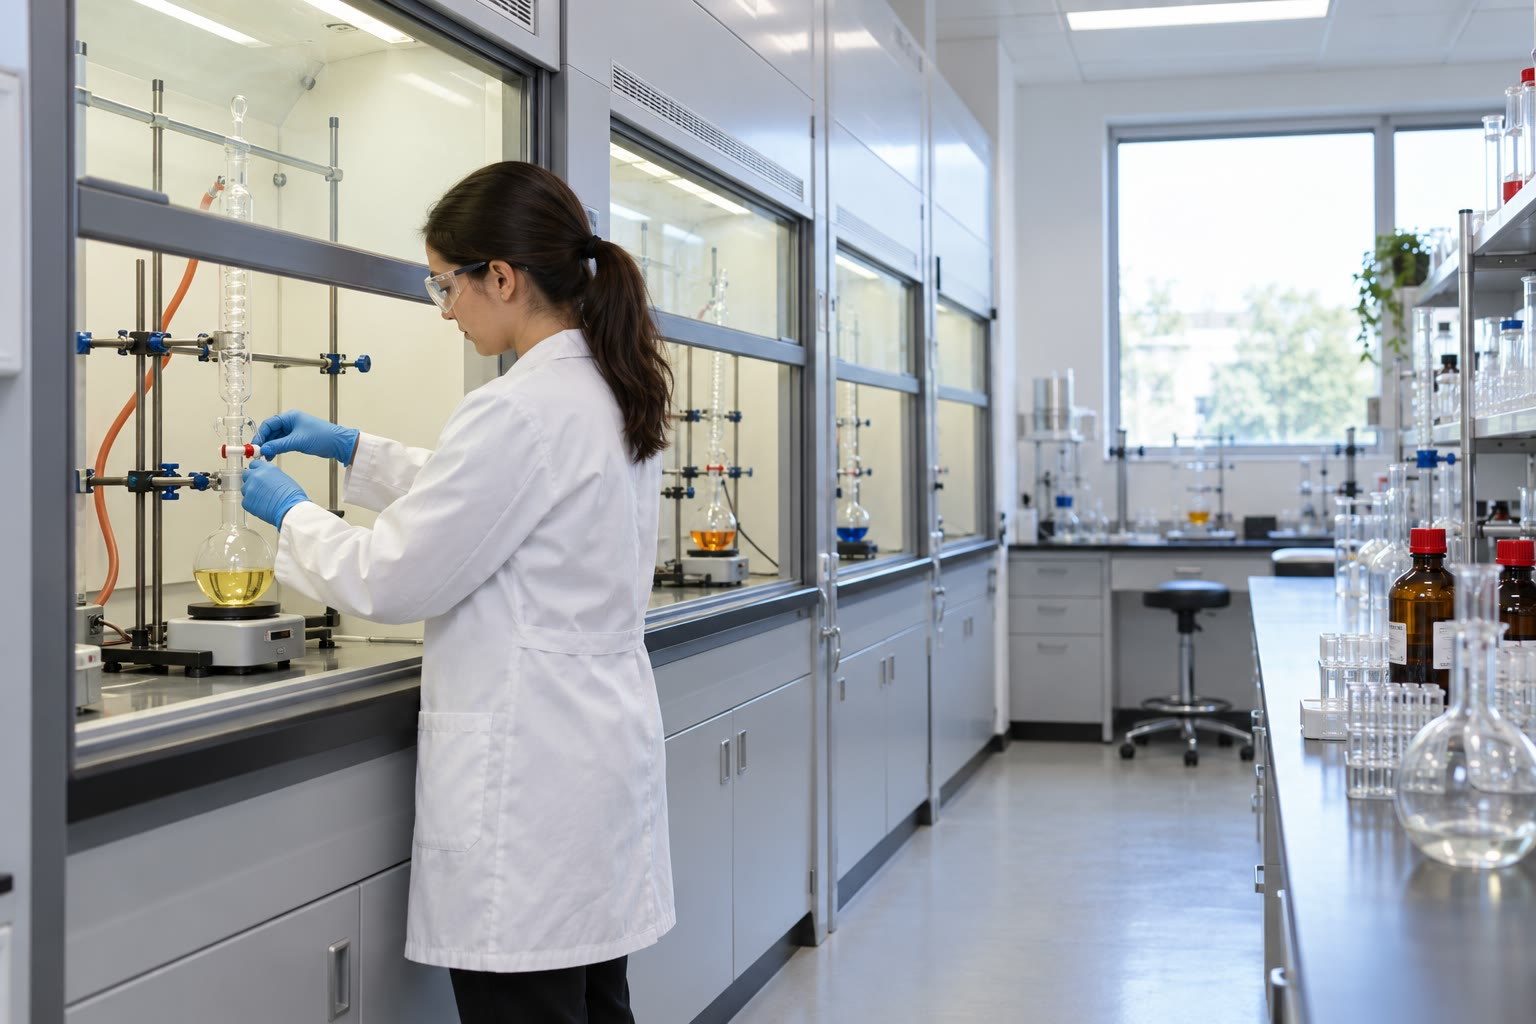
\includegraphics[width=0.56\linewidth]{images/book3/ai/b2-35-synthesis-lab.jpg}

{\small एक कार्बनिक संश्लेषण प्रयोगशाला: धूम-हुडों में चलती अभिक्रियाएँ, स्टैंडों पर कसे फ़्लास्क
(चित्रण)।}
\end{omfigure}

\begin{recall}
प्रथम वर्ष का खंड: संकट और GHS लेबल, निष्कर्षण, पुनःक्रिस्टलन, आसवन, पतली परत
\omterm{def:b2:chromatography:principle}{वर्णलेखन} और $R_f$, गलनांक, ग्रीन्यार अभिकर्मक। \Cref{ch:b2:reaction-enthalpy}: \omterm{def:b2:reaction-enthalpy:reaction-quantity}{अभिक्रिया
एन्थैल्पी} और \omterm{def:b2:continuous-reactors:adiabatic-rise}{रुद्धोष्म ताप-वृद्धि}। \Cref{ch:b2:chromatography},
\cref{ch:b2:structure-determination} और \cref{ch:b2:measurement-statistics}: विश्लेषण।
\end{recall}

\section{नियंत्रण में अभिक्रिया चलाना}

फ़्लास्क में कोई अभिक्रिया अपनी ऊष्मा वहीं मुक्त करती है जहाँ वह होती है। रसायनज्ञ ताप को एक कुंड
(बर्फ़ और जल, बर्फ़ और नमक, सबसे निम्न तापों के लिए शुष्क बर्फ़ और ऐसीटोन), किसी उबलते विलायक के
पश्चवाह से, जो संघनित्र द्वारा वाष्प लौटाते हुए ताप को उसके क्वथनांक पर सीमित कर देता है, और किसी अभिकर्मक को मिलाने की
दर से नियंत्रित करता है। एक आंतरिक तापमापी, कुंड के बजाय द्रव में, वही मापता है जो
महत्त्वपूर्ण है।

\begin{proposition}[संचयन]\label{prop:b2:lab-techniques-2:accumulation}
यदि कोई अभिकर्मक जितनी तेज़ी से अभिक्रिया करता है उससे तेज़ी से मिलाया जाए, तो अनभिक्रियित मात्रा $n_{\mathrm{acc}}$ संचित होती है। यदि
वह फिर एक साथ, बिना शीतन के, अभिक्रिया कर ले, तो ऊष्मा धारिता $C$ वाले मिश्रण का ताप इतना बढ़ता है:
\begin{equation*}
\Delta T_{\mathrm{ad}} = \frac{n_{\mathrm{acc}}\,|\Delta_rH|}{C}.
\end{equation*}
\end{proposition}

\begin{proof}
$n_{\mathrm{acc}}$ की अभिक्रिया नियत दाब पर $n_{\mathrm{acc}}|\Delta_rH|$ मुक्त करती है
(\cref{ch:b2:reaction-enthalpy}); ऊष्मा विनिमय के बिना यह सारी मिश्रण को गर्म करती है, जैसे
\omterm{def:b2:reaction-enthalpy:flame-temperature}{रुद्धोष्म ज्वाला ताप} में (\cref{def:b2:reaction-enthalpy:flame-temperature}): $C\Delta T =
n_{\mathrm{acc}}|\Delta_rH|$।
\end{proof}

ख़तरा तब सबसे अधिक होता है जब कोई अभिक्रिया आरंभ होने में धीमी हो, जैसे ग्रीन्यार निर्माण प्रायः होते हैं: आरंभन से पहले मिलाया गया
हैलाइड जमा होता जाता है, और जब अभिक्रिया अंततः आरंभ होती है तो वह अनियंत्रित हो जाती है। नियम यह है कि एक छोटा
भाग मिलाइए, अभिक्रिया को आरंभ होते देखिए (गर्माहट, धुँधलापन, हल्का पश्चवाह), और तभी शेष को
उस दर से मिलाइए जिसके साथ शीतन चल सके।

\section{शुष्क परिस्थितियाँ और अक्रिय वायुमंडल}

\begin{definition}[अक्रिय वायुमंडल]\label{def:b2:lab-techniques-2:inert}
कोई अभिक्रिया \emph{अक्रिय वायुमंडल}\index{अक्रिय वायुमंडल} के अंतर्गत चलाई जाती है जब उपकरण की वायु
को किसी अनभिक्रियाशील गैस, नाइट्रोजन या आर्गन, से प्रतिस्थापित कर दिया गया हो, जिसे हल्के अधिदाब पर रखा जाता है ताकि वायु
प्रवेश न कर सके।
\end{definition}

कार्बधात्विक अभिकर्मक, धातु हाइड्राइड और अनेक उत्प्रेरक जल और ऑक्सीजन से अभिक्रिया करते हैं। काँच के उपकरण
ओवन में सुखाकर गर्म अवस्था में ही जोड़े जाते हैं, या गैस की धारा के अंतर्गत ज्वाला से तपाए जाते हैं; विलायक शुष्क ख़रीदे जाते हैं या
जल से अभिक्रिया करने वाले किसी अभिकर्मक पर सुखाए जाते हैं; द्रव रबर सेप्टम से होकर सिरिंजों से स्थानांतरित किए जाते हैं।
गैस एक तेल बुदबुदक से होकर निकलती है, जो प्रवाह दिखाता है और वायु को वापस बहने से रोकता है।
सबसे संवेदनशील यौगिकों के लिए श्लेंक लाइन और ग्लवबॉक्स तृतीय वर्ष के खंड में आते हैं।

\begin{omfigure}
\begin{tikzpicture}[lab/.style={font=\scriptsize, align=center}]
\fill[omDef!10] (-1.7,-0.3) rectangle (1.7,1.0);
\draw[om glass] (-1.7,1.2) -- (-1.7,-0.3) -- (1.7,-0.3) -- (1.7,1.2);
\foreach \x/\y in {-1.5/0.0,-1.45/0.55,1.3/0.05,1.3/0.6,-1.25/0.3,1.05/-0.15}{
  \draw[omDef!50, fill=white] (\x,\y) rectangle ++(0.18,0.18);}
\pic (f) at (0,0) {threeneck={0.35}{omThm!25}};
\pic[rotate=25] (d) at (f-l) {dropfunnel={0.5}{omMeth!20}};
\pic (c) at (f-c) {condenser};
\pic[rotate=-25] (t) at (0.0,0.42) {thermometer};
\pic (b) at (3.6,3.6) {bubbler};
\draw[thick, black!60] (0,6.25) -- (0,6.75) -- (3.25,6.75) -- (b-in);
\coordinate (dtop) at ($(f-l)+(-1.52,3.26)$);
\draw[thick, black!60] (dtop) -- ++(0,0.35) -- ++(-0.9,0) node[left, lab] {N$_2$};
\node[lab, anchor=north] at (0,-0.4) {बर्फ़ कुंड};
\node[lab, anchor=east] at (-1.9,2.6) {योजक\\कीप};
\node[lab, anchor=west] at (0.55,5.0) {संघनित्र};
\node[lab, anchor=west] at (1.75,2.6) {तापमापी\\(आंतरिक)};
\node[lab, anchor=north] at (3.6,3.45) {बुदबुदक (गैस निकास)};
\end{tikzpicture}
\par\vspace{4pt}

{\small नाइट्रोजन के अंतर्गत एक अभिक्रिया (व्यवस्था-रूप)। बर्फ़ कुंड में तीन-मुँह वाला फ़्लास्क, द्रव में एक आंतरिक
तापमापी के साथ; अभिकर्मक एक दाब-समकारी कीप से मिलाया जाता है जिससे होकर
नाइट्रोजन प्रवेश करती है; गैस संघनित्र और एक तेल बुदबुदक से होकर निकलती है।}
\end{omfigure}

\begin{method}[नाइट्रोजन के अंतर्गत शुष्क अभिक्रिया की व्यवस्था]\label{met:b2:lab-techniques-2:anhydrous}
\begin{enumerate}
  \item काँच के उपकरण ओवन में सुखाइए और गर्म अवस्था में ही जोड़िए, जोड़ों पर ग्रीज़ या आस्तीन लगाकर; एक सेप्टम
        या योजक कीप, संघनित्र और बुदबुदक लगाइए।
  \item ठंडा होते समय नाइट्रोजन प्रवाहित कीजिए; पूरे समय धीमा प्रवाह (हर एक या दो सेकंड में एक बुलबुला) बनाए रखिए।
  \item ठोस प्रवाहन से पहले डालिए, शुष्क विलायक और द्रव अभिकर्मक किसी सेप्टम से होकर सिरिंज या कैन्युला से।
  \item योजना के अनुसार ठंडा या गर्म कीजिए; एक छोटे भाग से योजन आरंभ कीजिए और आगे बढ़ने से पहले जाँचिए कि अभिक्रिया
        आरंभ हो गई है।
\end{enumerate}
\end{method}

\section{उपचार-पश्चात् प्रक्रिया}

\begin{definition}[उपचार-पश्चात् प्रक्रिया]\label{def:b2:lab-techniques-2:work-up}
किसी अभिक्रिया की \emph{उपचार-पश्चात् प्रक्रिया}\index{उपचार-पश्चात् प्रक्रिया} अभिक्रिया के बाद की संक्रियाओं का वह अनुक्रम है जो
अभिक्रिया मिश्रण को अपरिष्कृत उत्पाद में बदलता है: शमन, निष्कर्षण और धुलाई, शुष्कन,
निस्यंदन और विलायक का वाष्पन।
\end{definition}

\begin{definition}[अम्ल--क्षारक निष्कर्षण]\label{def:b2:lab-techniques-2:acid-base-extraction}
\emph{अम्ल--क्षारक निष्कर्षण}\index{अम्ल--क्षारक निष्कर्षण} किसी कार्बनिक विलायक में घुले अम्लीय, क्षारकीय और उदासीन कार्बनिक
यौगिकों को विलयन को जलीय अम्लों या क्षारकों से धोकर पृथक करता है, जो
यौगिकों के एक वर्ग को ऐसे आयनों में बदल देते हैं जो जल में चले जाते हैं।
\end{definition}

\begin{proposition}[कौन कहाँ जाता है]\label{prop:b2:lab-techniques-2:acid-base-extraction}
जलीय सोडियम हाइड्रोजनकार्बोनेट (pH 8.3) किसी कार्बोक्सिलिक अम्ल ($\mathrm pK_a$ लगभग 4) का निष्कर्षण करता है परंतु किसी
फ़ीनॉल ($\mathrm pK_a$ लगभग 10) का नहीं, जिसके लिए सोडियम हाइड्रॉक्साइड चाहिए; तनु हाइड्रोक्लोरिक अम्ल ऐसे
ऐमीन का निष्कर्षण करता है जिसके संयुग्मी अम्ल का $\mathrm pK_a$ 4.6 या अधिक हो; उदासीन यौगिक कार्बनिक
परत में रहते हैं।
% ledger: ph:NaHCO3, pka:benzoic, pka:phenol, pka:anilinium
\end{proposition}

\begin{proof}
कोई स्पीशीज़ मुख्यतः अपने क्षारकीय रूप में होती है जब $\mathrm{pH} > \mathrm pK_a$, और 99~\% से अधिक तब जब
$\mathrm{pH} > \mathrm pK_a + 2$। pH 8.3 पर बेन्ज़ोइक अम्ल (4.2) 99~\% से अधिक बेन्ज़ोएट है, एक आयन
जो जल में रहता है; फ़ीनॉल (9.99) लगभग 2~\% फ़ीनॉक्साइड है ($10^{8.3 - 10.0}$) और अनिवार्यतः
कार्बनिक परत में रहता है, जहाँ उदासीन रूप का विभाजन होता है। सोडियम हाइड्रॉक्साइड (pH 12 से ऊपर) में फ़ीनॉल
फ़ीनॉक्साइड में बदल जाता है। तनु हाइड्रोक्लोरिक अम्ल (pH लगभग 1) में ऐनिलीन (ऐनिलीनियम 4.6) 99~\% से अधिक
ऐनिलीनियम है। हर आयन, जल में पहुँचने के बाद, pH को उलटी ओर लौटाकर पुनः प्राप्त किया जाता है, जो
उदासीन यौगिक का पुनर्जनन करता है, फिर उसका फिर से निष्कर्षण किया जाता है।
\end{proof}

\begin{omfigure}
\begin{tikzpicture}[x=1cm, y=1cm, st/.style={draw=black!70, rounded corners=2pt, fill=white,
  font=\scriptsize, align=center, inner sep=3pt, text width=3.0cm}, ar/.style={->, thick, black!70}]
\node[st, fill=omDef!10] (m) at (0,0) {बेन्ज़ोइक अम्ल, फ़ीनॉल,\\ऐनिलीन, नैफ़्थलीन\\एथॉक्सीएथेन में};
\node[st, fill=omThm!10] (a1) at (5.0,0) {जलीय: बेन्ज़ोएट\\$\to$ HCl $\to$ बेन्ज़ोइक अम्ल};
\node[st] (o1) at (0,-1.6) {फ़ीनॉल, ऐनिलीन,\\नैफ़्थलीन};
\node[st, fill=omThm!10] (a2) at (5.0,-1.6) {जलीय: फ़ीनॉक्साइड\\$\to$ HCl $\to$ फ़ीनॉल};
\node[st] (o2) at (0,-3.2) {ऐनिलीन, नैफ़्थलीन};
\node[st, fill=omThm!10] (a3) at (5.0,-3.2) {जलीय: ऐनिलीनियम\\$\to$ NaOH $\to$ ऐनिलीन};
\node[st, fill=omMeth!10] (o3) at (0,-4.8) {नैफ़्थलीन\\(सुखाइए, वाष्पित कीजिए)};
\draw[ar] (m) -- node[above, font=\tiny] {NaHCO$_3$ धुलाई} (a1);
\draw[ar] (m) -- (o1); \draw[ar] (o1) -- node[above, font=\tiny] {NaOH धुलाई} (a2);
\draw[ar] (o1) -- (o2); \draw[ar] (o2) -- node[above, font=\tiny] {HCl धुलाई} (a3);
\draw[ar] (o2) -- (o3);
\pic at (8.6,-3.6) {sepfunnel={omDef!25}{omThm!20}};
\node[font=\scriptsize, align=center] at (8.6,-4.0) {पृथक्कारी कीप};
\end{tikzpicture}
\par\vspace{4pt}

{\small चार यौगिकों का अम्ल--क्षारक पृथक्करण (\cref{prop:b2:lab-techniques-2:acid-base-extraction})।
कार्बनिक परत (बायाँ स्तंभ) हर धुलाई में एक वर्ग खोती है; हर जलीय निष्कर्ष (दायाँ) pH उलटने पर
अपना यौगिक लौटा देता है।}
\end{omfigure}

\begin{definition}[शुष्कन कारक]\label{def:b2:lab-techniques-2:drying-agent}
\emph{शुष्कन कारक}\index{शुष्कन कारक} कोई निर्जल लवण है, जैसे मैग्नीशियम या सोडियम सल्फ़ेट,
जो किसी कार्बनिक विलयन में घुले जल को जलयोजन जल के रूप में बाँध लेता है और फिर
निस्यंदन से हटा दिया जाता है।
\end{definition}

\begin{method}[अभिक्रिया फ़्लास्क से अपरिष्कृत उत्पाद तक]\label{met:b2:lab-techniques-2:work-up}
\begin{enumerate}
  \item शमन: शेष अभिक्रियाशील अभिकर्मकों को किसी उपयुक्त जलीय विलयन से, धीरे-धीरे और
        ठंडा करते हुए, नष्ट कीजिए।
  \item किसी कार्बनिक विलायक में निष्कर्षित कीजिए; परतों को अलग कीजिए (कौन-सी कौन है यह जल की एक बूँद
        डालकर जाँचिए); जलीय परत का फिर से निष्कर्षण कीजिए।
  \item संयुक्त कार्बनिक परतों को धोइए (अम्ल, क्षारक, फिर लवण-जल, अर्थात् सोडियम क्लोराइड का संतृप्त विलयन
        जो घुले जल का अधिकांश भाग हटा देता है)।
  \item \omterm{def:b2:lab-techniques-2:drying-agent}{शुष्कन कारक} से तब तक सुखाइए जब तक उसका कुछ भाग मुक्त-प्रवाही न रहे; छानिए।
  \item घटे हुए दाब पर घूर्णी वाष्पित्र में विलायक हटाइए; अपरिष्कृत उत्पाद को तौलिए।
\end{enumerate}
\end{method}

\section{शोधन}

\begin{definition}[फ़्लैश वर्णलेखन]\label{def:b2:lab-techniques-2:flash}
\emph{फ़्लैश वर्णलेखन}\index{फ़्लैश वर्णलेखन} सिलिका पर किया जाने वाला प्रारंभिक स्तंभ \omterm{def:b2:chromatography:principle}{वर्णलेखन} है जिसमें
निक्षालक को हल्के गैस दाब से स्तंभ से होकर धकेला जाता है, जिससे ग्रामों पदार्थ का पृथक्करण
मिनटों में हो जाता है; निक्षालक उसी सिलिका पर पतली परत \omterm{def:b2:chromatography:principle}{वर्णलेखन} से चुना जाता है।
\end{definition}

\begin{proposition}[स्तंभ आयतन]\label{prop:b2:lab-techniques-2:column-volumes}
जो यौगिक किसी TLC प्लेट पर $R_f$ पर चलता है, वह उसी सिलिका और निक्षालक वाले स्तंभ से
निक्षालक के लगभग $1/R_f$ स्तंभ आयतनों के बाद निकलता है।
\end{proposition}

\begin{proof}[तर्क]
प्लेट पर यौगिक विलायक अग्र से $R_f$ गुना दूरी तय करता है: उसकी औसत चाल निक्षालक की चाल का
$R_f$ गुना है। स्तंभ पर वही विभाजन चालों का वही अनुपात देता है, अतः
यौगिक को बाहर आने के लिए स्तंभ को भरने वाले निक्षालक के आयतन (मृत आयतन) का $1/R_f$ गुना
चाहिए; \cref{ch:b2:chromatography} की भाषा में $R_f \approx 1/(1 + k)$। $R_f = 0.25$ पर कोई यौगिक
लगभग चार स्तंभ आयतनों के बाद निकलता है, 0.5 वाले (दो आयतन) से भली-भाँति पृथक।
\end{proof}

\begin{omfigure}
\begin{tikzpicture}[lab/.style={font=\scriptsize, align=left, anchor=west}]
\pic (k) at (0,0) {chromcolumn={3.4}};
\node[lab] at (0.6,4.6) {निक्षालक};
\node[lab] at (0.6,3.55) {रेत};
\node[lab] at (0.6,2.2) {सिलिका संस्तर};
\foreach \i/\c in {0/white, 1/omThm!25, 2/omThm!25, 3/white, 4/omDef!25, 5/omDef!25, 6/white}{
  \pic at ({2.4+0.55*\i},-1.2) {testtube={0.45}{\c}};}
\node[font=\scriptsize] at (4.05,-1.6) {अंश 1 से 7};
\pic at (7.6,-1.2) {tlcplate};
\foreach \j/\x in {2/7.15,3/7.45,5/7.75,6/8.05}{\node[font=\tiny] at (\x,-1.38) {\j};}
\fill[omThm] (7.45,0.95) circle (0.06); \fill[omThm] (7.15,0.95) circle (0.06);
\fill[omDef] (8.05,-0.05) circle (0.06); \fill[omDef] (7.75,-0.05) circle (0.06);
\node[font=\scriptsize, align=center] at (7.6,2.15) {अंशों का\\TLC};
\end{tikzpicture}
\par\vspace{4pt}

{\small \omterm{def:b2:lab-techniques-2:flash}{फ़्लैश वर्णलेखन} (व्यवस्था-रूप)। अपरिष्कृत उत्पाद को सिलिका के ऊपर रखकर उत्क्षालित किया जाता है;
उत्क्षालित द्रव को अंशों में एकत्र किया जाता है; अंशों की एक TLC प्लेट दिखाती है कि हर यौगिक कहाँ निकला
(यहाँ तेज़, अध्रुवी यौगिक अंश 2--3 में, धीमा 5--6 में), और शुद्ध अंशों को
मिला दिया जाता है।}
\end{omfigure}

\begin{method}[फ़्लैश स्तंभ चलाना]\label{met:b2:lab-techniques-2:flash}
\begin{enumerate}
  \item TLC द्वारा निक्षालक चुनिए: वांछित यौगिक $R_f$ लगभग 0.25--0.35 पर, अशुद्धियों से यथासंभव
        दूर।
  \item सिलिका (अपरिष्कृत उत्पाद के द्रव्यमान का लगभग 30 से 100 गुना) को घोल के रूप में या शुष्क भरिए; रेत की एक परत
        डालिए।
  \item अपरिष्कृत उत्पाद को विलायक के न्यूनतम आयतन में (या थोड़े सिलिका पर अधिशोषित करके) डालिए।
  \item हल्के दाब में उत्क्षालित कीजिए; अंश एकत्र कीजिए; TLC से उनकी जाँच कीजिए; शुद्ध अंशों को मिलाकर
        वाष्पित कीजिए।
\end{enumerate}
\end{method}

जो द्रव अपने क्वथनांक के निकट विघटित हो जाते हैं, उन्हें घटे हुए दाब पर आसवित किया जाता है, जहाँ वे
कम ताप पर उबलते हैं।

\begin{definition}[घटे हुए दाब पर आसवन]\label{def:b2:lab-techniques-2:reduced-pressure}
\emph{घटे हुए दाब पर आसवन}\index{घटे हुए दाब पर आसवन} ऐसे उपकरण में किया जाता है
जो एक दाबमापी से होकर निर्वात पंप से जुड़ा हो, ऐसे दाब पर जहाँ द्रव
किसी ऐसे ताप पर उबलता है जिसे वह सह सके।
\end{definition}

\begin{proposition}[घटे हुए दाब पर क्वथन]\label{prop:b2:lab-techniques-2:reduced-pressure}
क्वथन ताप $T_b$ के साथ, संदर्भ दाब $p^\circ$ पर, और $\Delta_{\mathrm{vap}}H$ को
नियत मानकर, दाब $p$ पर क्वथन ताप इससे दिया जाता है:
\begin{equation*}
\frac{1}{T} = \frac{1}{T_b} - \frac{R}{\Delta_{\mathrm{vap}}H}\ln\frac{p}{p^\circ}.
\end{equation*}
\end{proposition}

\begin{proof}
कोई द्रव तब उबलता है जब उसका वाष्प दाब उसके ऊपर के दाब के बराबर हो जाता है। भौतिकी का क्लॉसियस--क्लेपेरॉन संबंध,
आदर्श वाष्प और नगण्य द्रव आयतन के लिए $\mathrm d\ln p/\mathrm dT = \Delta_{\mathrm{vap}}H/(RT^2)$,
$(T_b, p^\circ)$ और $(T, p)$ के बीच समाकलित होकर $\ln(p/p^\circ) =
-(\Delta_{\mathrm{vap}}H/R)(1/T - 1/T_b)$ देता है; पुनर्व्यवस्थित करने पर परिणाम मिलता है।
\end{proof}

\begin{omfigure}
\begin{tikzpicture}
\begin{axis}[width=0.72\linewidth, height=5.2cm, xmode=log, xmin=5, xmax=1100, ymin=0, ymax=190,
  xlabel={दाब (\unit{mbar})}, ylabel={क्वथन ताप (\unit{\degreeCelsius})},
  label style={font=\small}, tick label style={font=\scriptsize}, grid=major, grid style={black!10},
  legend style={font=\scriptsize, at={(0.02,0.98)}, anchor=north west}, legend cell align=left]
\addplot[omDef, thick] table[x=p, y=bromobenzene] {figdata/out/bachelor-2-vacuum-boiling.dat};
\addplot[omThm, thick] table[x=p, y=benzaldehyde] {figdata/out/bachelor-2-vacuum-boiling.dat};
\addplot[only marks, mark=o, mark size=2pt, omDef] coordinates {(7,27.75)};
\addplot[only marks, mark=o, mark size=2pt, omThm] coordinates {(13,61.85)};
\legend{ब्रोमोबेन्ज़ीन, बेन्ज़ैल्डिहाइड, मापित}
\end{axis}
\end{tikzpicture}

{\small दाब के विरुद्ध क्वथन ताप (\cref{prop:b2:lab-techniques-2:reduced-pressure}),
NIST वेबबुक की वाष्पन एन्थैल्पियों और क्वथनांकों के साथ। वृत्त 7 और \qty{13}{mbar} पर मापे गए क्वथनांक
हैं, जो वक्रों में प्रयुक्त नहीं हुए: सरल समीकरण कुछ केल्विन के भीतर है।
दाब को \qty{1}{bar} से \qty{20}{mbar} तक घटाने से क्वथनांक
\qty{100}{K} से अधिक गिर जाते हैं।}
% figdata: bachelor-2/vacuum-boiling.py
% ledger: tb:bromobenzene, dvap:bromobenzene, tbp:bromobenzene.7mbar, tb:benzaldehyde, dvap:benzaldehyde, tbp:benzaldehyde.13mbar
\end{omfigure}

\section{शुद्धता और पहचान}

किसी उत्पाद की पहचान उसके स्पेक्ट्रमों और भौतिक स्थिरांकों की अपेक्षित
यौगिक के स्पेक्ट्रमों और स्थिरांकों से तुलना करके होती है (\cref{ch:b2:structure-determination}); उसकी शुद्धता अलग से मापी जाती है, क्योंकि कोई उत्पाद
सही यौगिक होते हुए भी किसी अन्य पदार्थ का कई प्रतिशत रख सकता है।

\begin{method}[शुद्धता और लब्धि बताना]\label{met:b2:lab-techniques-2:purity}
\begin{enumerate}
  \item किसी ठोस का गलन परास (शुद्ध यौगिक के लिए तीक्ष्ण और साहित्य मान के निकट) और उसका
        TLC (दो निक्षालकों में एक धब्बा) जाँचिए।
  \item शुद्धता मापिए: GC या HPLC में क्षेत्रफल प्रतिशत (केवल एक अनुमान, जब तक \omterm{def:b2:chromatography:quantitative}{अनुक्रिया गुणांक} ज्ञात न हों,
        \cref{ch:b2:chromatography}), या मात्रात्मक प्रोटॉन NMR, उत्पाद के किसी समाकल की
        हर अशुद्धि के किसी समाकल से, या तौले गए \omterm{def:b2:chromatography:quantitative}{आंतरिक मानक} से तुलना करके।
  \item पृथक्कृत पदार्थ में उत्पाद के द्रव्यमान अंश $w$ में बदलिए।
  \item शुद्धता के लिए संशोधित लब्धि बताइए: $\rho = w\,m/(n_{\mathrm{lim}}M)$, जहाँ $m$
        पृथक्कृत द्रव्यमान है, $n_{\mathrm{lim}}$ सीमांत अभिकर्मक की मात्रा और $M$ मोलर द्रव्यमान।
\end{enumerate}
\end{method}

किसी प्रकाशिक सक्रिय उत्पाद के लिए विशिष्ट घूर्णन उसकी त्रिविम-रासायनिक शुद्धता की एक जाँच जोड़ता है;
प्रतिबिंबरूपी आधिक्य और उसके मापन का विवेचन तृतीय वर्ष के खंड में है।

\begin{safety}{\ghs[5mm]{GHS02}\,\ghs[5mm]{GHS06}\,\ghs[5mm]{GHS07}\,\ghs[5mm]{GHS08}\,\ghs[5mm]{GHS09}}
एथॉक्सीएथेन और ऑक्सोलेन अत्यंत ज्वलनशील हैं और भंडारण में विस्फोटक परॉक्साइड बनाते हैं; प्रयोगशाला में
कोई ज्वाला नहीं, पुरानी बोतलों का आसवन से पहले परीक्षण कीजिए। ब्रोमोबेन्ज़ीन ज्वलनशील और जलीय जीवों के लिए
विषैला है; मैग्नीशियम की छीलन ज्वलनशील है। निर्वात काँच-उपकरणों में तारकाकार दरारों की जाँच की जाती है और उन्हें परिरक्षित किया जाता है।
% ledger: ghs:ether, ghs:THF, ghs:bromobenzene, ghs:Mg, ghs:MgSO4
\end{safety}

\section{अभ्यास}

\begin{exercise}[$\star$]\label{exo:b2:lab-techniques-2:1}
लगभग \qty{0}{\degreeCelsius} पर, लगभग
\qty{-15}{\degreeCelsius} पर, और \qty{-78}{\degreeCelsius} पर चलाई जाने वाली अभिक्रिया के लिए आप कौन-सा कुंड प्रयुक्त करेंगे?
\end{exercise}

\begin{exercise}[$\star$]\label{exo:b2:lab-techniques-2:2}
कोई निष्कर्षण डाइक्लोरोमेथेन प्रयुक्त करता है, जो जल से सघन है। कौन-सी परत कार्बनिक है? आप कैसे जाँचेंगे?
\end{exercise}

\begin{exercise}[$\star$]\label{exo:b2:lab-techniques-2:3}
आप कैसे जानेंगे कि किसी ईथर विलयन में पर्याप्त मैग्नीशियम सल्फ़ेट मिला दिया गया है?
\end{exercise}

\begin{exercise}[$\star$]\label{exo:b2:lab-techniques-2:4}
4\,:\,1 हेक्सेन--एथिल ऐसीटेट में किसी उत्पाद का $R_f = 0.65$ है और किसी अशुद्धि का 0.75। स्तंभ के लिए आप क्या
बदलेंगे, और किस दिशा में?
\end{exercise}

\begin{exercise}[$\star\star$]\label{exo:b2:lab-techniques-2:5}
बेन्ज़ोइक अम्ल, फ़ीनॉल, ऐनिलीन और नैफ़्थलीन को किसी ईथर विलयन से पृथक करने वाली धुलाइयों का क्रम दीजिए,
हर एक को किसी $\mathrm pK_a$ से उचित ठहराते हुए, और यह भी कि हर यौगिक कैसे पुनः प्राप्त होता है।
\end{exercise}

\begin{exercise}[$\star\star$]\label{exo:b2:lab-techniques-2:6}
\qty{20}{mbar} पर ब्रोमोबेन्ज़ीन और बेन्ज़ैल्डिहाइड के क्वथन तापों का आकलन कीजिए।
\end{exercise}

\begin{exercise}[$\star\star$]\label{exo:b2:lab-techniques-2:7}
किसी योजन के दौरान किसी अभिकर्मक का \qty{0.050}{mol} अनभिक्रियित रूप में संचित हो गया है। $\Delta_rH =
\qty{-200}{kJ/mol}$ और मिश्रण की ऊष्मा धारिता \qty{400}{J/K} के साथ (अभ्यास के आँकड़े), इसके बाद
ताप में कितनी वृद्धि हो सकती है?
\end{exercise}

\begin{exercise}[$\star\star$]\label{exo:b2:lab-techniques-2:8}
एक HPLC अनुरेख उत्पाद को कुल क्षेत्रफल के 96.0~\% पर दिखाता है। यह अभी द्रव्यमान शुद्धता क्यों नहीं है? उसी नमूने का
एक प्रोटॉन स्पेक्ट्रम समाकल 1.00 वाला एक उत्पाद एकक (1H) और समाकल 0.12 वाला एक अशुद्धि एकक
(3H) दिखाता है; उत्पाद \qty{200}{g/mol}, अशुद्धि \qty{100}{g/mol} (अभ्यास के आँकड़े)। उत्पाद का
द्रव्यमान अंश परिकलित कीजिए।
\end{exercise}

\begin{exercise}[$\star\star$]\label{exo:b2:lab-techniques-2:9}
\qty{0.0300}{mol} सीमांत अभिकर्मक से 95.0~\% (द्रव्यमान) शुद्धता वाले किसी उत्पाद (\qty{164}{g/mol}) के \qty{4.10}{g}
प्राप्त होते हैं। लब्धि परिकलित कीजिए, असंशोधित और संशोधित।
\end{exercise}

\begin{exercise}[$\star\star\star$]\label{exo:b2:lab-techniques-2:10}
ऐल्डिहाइड मिलाने के बाद एक ग्रीन्यार अभिक्रिया ने बेन्ज़ीन दी और लगभग कोई ऐल्कोहॉल नहीं। संभावित
कारणों की सूची बनाइए और बताइए कि हर एक से कैसे बचा जाए।
\end{exercise}

\begin{exercise}[$\star\star\star$]\label{exo:b2:lab-techniques-2:11}
पैमाना बढ़ाने पर किसी हैलाइड का \qty{1.00}{mol} $\Delta_rH = \qty{-270}{kJ/mol}$ के साथ ऐसे रिएक्टर में अभिक्रिया करता है जिसका
शीतन अधिकतम \qty{150}{W} हटाता है (अभ्यास के आँकड़े)। सबसे छोटा सुरक्षित योजन समय क्या है? यदि योजन
तेज़ हो तो क्या होता है?
\end{exercise}

\begin{exercise}[$\star\star\star$]\label{exo:b2:lab-techniques-2:12}
\qty{13.0}{g} का कोई अपरिष्कृत ठोस पुनःक्रिस्टलन (एक चरण, 80~\% पुनर्प्राप्ति, शुद्धता
99~\%) या \omterm{def:b2:lab-techniques-2:flash}{फ़्लैश वर्णलेखन} (95~\% पुनर्प्राप्ति, शुद्धता 99.5~\%, विलायक का \qty{1.5}{L}) द्वारा शोधित किया जा सकता है (अभ्यास के
आँकड़े)। दोनों मार्गों की तुलना कीजिए।
\end{exercise}

\section{समस्या: ठीक ढंग से किया गया एक ग्रीन्यार}

\begin{problem}[{सप्ताहांत समस्या --- संकट और शुष्क व्यवस्था, नियंत्रित योजन और
संचयन का ख़तरा, उपचार-पश्चात् प्रक्रिया, फ़्लैश वर्णलेखन द्वारा शोधन और शुद्धता-संशोधित लब्धि}]
\label{pb:b2:lab-techniques-2:1}
अभ्यास के आँकड़े। ब्रोमोबेन्ज़ीन के \qty{15.7}{g} और मैग्नीशियम छीलन के \qty{2.67}{g} से शुष्क एथॉक्सीएथेन में
फ़ेनिलमैग्नीशियम ब्रोमाइड बनाया जाता है, फिर बेन्ज़ैल्डिहाइड का \qty{9.55}{g} मिलाया जाता है; जलीय अमोनियम क्लोराइड के साथ
\omterm{def:b2:lab-techniques-2:work-up}{उपचार-पश्चात् प्रक्रिया} डाइफ़ेनिलमेथेनॉल देती है। अभिकर्मक का बनना: $\Delta_rH =
\qty{-270}{kJ/mol}$; मिश्रण की ऊष्मा धारिता \qty{170}{J/K}; आरंभ \qty{20}{\degreeCelsius} पर। TLC
(9\,:\,1 हेक्सेन--एथिल ऐसीटेट): बाइफ़ेनिल $R_f = 0.85$, डाइफ़ेनिलमेथेनॉल 0.25। स्तंभ के बाद पृथक्कृत:
\qty{12.50}{g}। इस पदार्थ का प्रोटॉन NMR: \ce{CH(OH)} एकक (1H) का समाकल 1.00, \omterm{def:b2:huckel:aromatic}{ऐरोमैटिक}
क्षेत्र 10.90। मोलर द्रव्यमान (\unit{g/mol}): ब्रोमोबेन्ज़ीन 157.01, बेन्ज़ैल्डिहाइड 106.12, डाइफ़ेनिलमेथेनॉल
184.24, बाइफ़ेनिल 154.21; Mg 24.305।
% ledger: ghs:ether, ghs:bromobenzene, ghs:Mg, ghs:benzaldehyde, ghs:NH4Cl, ghs:biphenyl, ghs:benzhydrol, tb:ether, aw:Mg, aw:C, aw:H, aw:Br, aw:O, nmr:biphenyl

\medskip
\noindent\textbf{भाग I --- संकट और व्यवस्था।}
\begin{enumerate}
  \item एथॉक्सीएथेन, ब्रोमोबेन्ज़ीन और मैग्नीशियम के मुख्य संकट बताइए।
  \item जल के साथ फ़ेनिलमैग्नीशियम ब्रोमाइड की अभिक्रिया लिखिए, और ओवन में सुखाए गए काँच-उपकरणों की व्याख्या कीजिए।
  \item नाइट्रोजन के अंतर्गत काम क्यों करें?
  \item बुदबुदक क्या दिखाता है, और क्या रोकता है?
  \item यहाँ एथॉक्सीएथेन एक अच्छा विलायक क्यों है?
  \item ब्रोमोबेन्ज़ीन और मैग्नीशियम की मात्राएँ परिकलित कीजिए। कौन आधिक्य में है?
\end{enumerate}

\medskip
\noindent\textbf{भाग II --- नियंत्रित योजन।}
\begin{enumerate}[resume]
  \item अभिकर्मक का पूर्ण निर्माण कितनी ऊष्मा मुक्त करता है?
  \item ब्रोमोबेन्ज़ीन को बूँद-बूँद क्यों मिलाया जाता है?
  \item अभिक्रिया आरंभ होने में धीमी है, और उसके आरंभ होने से पहले ब्रोमोबेन्ज़ीन का 20~\% मिला दिया जाता है। तब एक साथ
        कितनी ऊष्मा मुक्त हो सकती है?
  \item \omterm{def:b2:continuous-reactors:adiabatic-rise}{रुद्धोष्म ताप-वृद्धि} परिकलित कीजिए।
  \item अंतिम ताप की तुलना एथॉक्सीएथेन के क्वथनांक से कीजिए। क्या होता है?
  \item योजन कैसे किया जाना चाहिए?
\end{enumerate}

\medskip
\noindent\textbf{भाग III --- योजन और \omterm{def:b2:lab-techniques-2:work-up}{उपचार-पश्चात् प्रक्रिया}।}
\begin{enumerate}[resume]
  \item बेन्ज़ैल्डिहाइड के साथ अभिक्रिया लिखिए और सीमांत अभिकर्मक पहचानिए।
  \item प्रबल अम्ल के बजाय अमोनियम क्लोराइड से शमन क्यों करें?
  \item पृथक्कारी कीप में कौन-सी परत कार्बनिक है?
  \item लवण-जल से धुलाई किसलिए है?
  \item विलयन को कैसे सुखाया जाता है, और विलायक को कैसे हटाया जाता है?
  \item बाइफ़ेनिल मुख्य उपोत्पाद है। यह कैसे बनता है, और इसे क्या बढ़ावा देता है?
\end{enumerate}

\medskip
\noindent\textbf{भाग IV --- शोधन और शुद्धता।}
\begin{enumerate}[resume]
  \item कौन-सा यौगिक स्तंभ से पहले निकलता है?
  \item हर एक कितने स्तंभ आयतनों के बाद निकलता है?
  \item NMR समाकलों से पृथक्कृत पदार्थ में बाइफ़ेनिल और ऐल्कोहॉल का मोलर अनुपात
        परिकलित कीजिए।
  \item डाइफ़ेनिलमेथेनॉल का द्रव्यमान अंश परिकलित कीजिए।
  \item शुद्ध डाइफ़ेनिलमेथेनॉल का द्रव्यमान परिकलित कीजिए।
  \item सैद्धांतिक द्रव्यमान परिकलित कीजिए।
  \item शुद्धता के लिए संशोधन के बिना लब्धि परिकलित कीजिए।
  \item शुद्धता के लिए संशोधित लब्धि बताइए।
\end{enumerate}
\end{problem}
